\documentclass{article}
\usepackage[utf8]{inputenc}
\usepackage{graphicx}
\graphicspath{ {Images/} }

\title{PS6_Cocklin}
\author{connorcocklin }
\date{March,5 2019}

\begin{document}

\section{First Visualization}
\includegraphics{Wordcloud}
\\[12pt]
I used an R script to initially find and create a csv file and then I cleaned up the table of NBA stats by deleting rows and columns until I was left with the raw data that was cleaned and necessary. It was impossible for me to figure out how to change the columns from character to numeric even with "as.numeric" syntax. So I cleaned that part in excel. After reading the data back in I created a wordcloud that showed the largest name as the highest ranking Player Efficiency Rating. I could have done a better job on the contrast in size because it is somewhat difficult to see that Anthony Davis is the leader.



\section{Second Visualization}
\includegraphics{CorrelationMatrix}
\\[12pt]
Here I created a correlation matrix that looked to see how the variables influence each other. This will lead me to my final Visualization because I saw that estimated wins added and player efficiency rating were highly correlated

\section{Third Visualization}
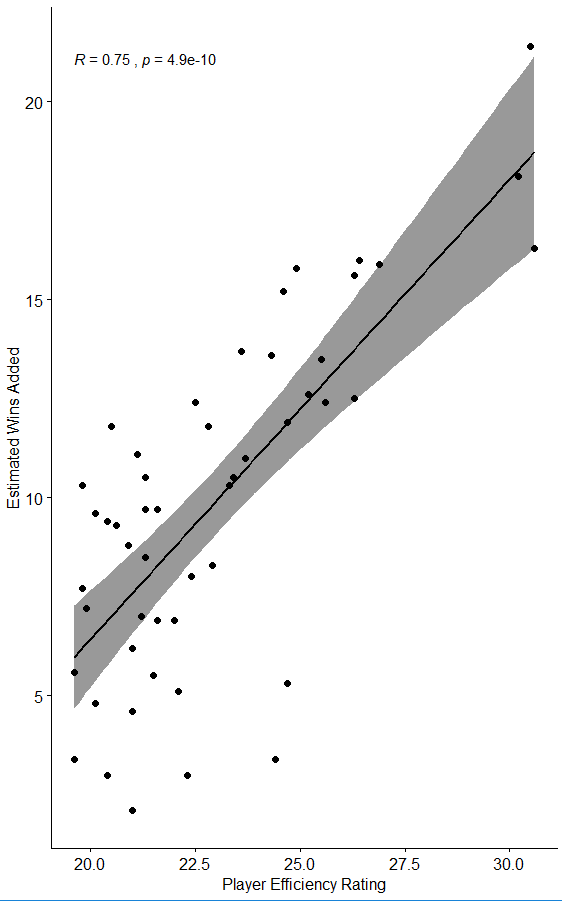
\includegraphics{PS6c_Cocklin}
\\[12pt]
This is a straight scatterplot correlation between Estimated Wins Added and Player Efficiency Rating between the top 50 ranked player by PER. I believe that these are so highly correlated because they share statistical similarities in how they are calculated. 
\end{document}
